%%%%%%%%%%%%%%%%%%%%%%%%%%%%%%%%%%%%%%%%%
% Fancyslides Presentation
% LaTeX Template
% Version 1.0 (30/6/13)
%
% This template has been downloaded from:
% http://www.LaTeXTemplates.com
%
% The Fancyslides class was created by:
% Paweł Łupkowski (pawel.lupkowski@gmail.com)
%
% License:
% CC BY-NC-SA 3.0 (http://creativecommons.org/licenses/by-nc-sa/3.0/)
%
%%%%%%%%%%%%%%%%%%%%%%%%%%%%%%%%%%%%%%%%%

%----------------------------------------------------------------------------------------
% PACKAGES AND OTHER DOCUMENT CONFIGURATIONS
%----------------------------------------------------------------------------------------

\title{make_Pa}
\documentclass{fancyslides}

\usepackage{graphicx, array, blindtext}

\usepackage[utf8]{inputenc} % Allows the usage of non-english characters
\usepackage{times} % Use the Times font
\usepackage{booktabs} % Allows the use of \toprule, \midrule and \bottomrule in tables
\graphicspath{{images/}} % Location of the slide background and figure files

% Beamer options - do not change
\usetheme{default} 
\setbeamertemplate{navigation symbols}{} % Disable the slide navigation buttons on the bottom of each slide
\setbeamercolor{structure}{fg=\yourowntexcol} % Define the color of titles and fixed text elements (e.g. bullet points)
\setbeamercolor{normal text}{fg=\yourowntexcol} % Define the color of text in the presentation

%------------------------------------------------
% COLORS
% The following colors are predefined in this class: white, black, gray, blue, green and orange

% Define your own color as follows:
%\definecolor{pink}{rgb}{156,0,151}

\newcommand{\structureopacity}{0.75} % Opacity (transparency) for the structure elements (boxes and circles)

\newcommand{\strcolor}{blue} % Set the color of structure elements (boxes and circles)
\newcommand{\yourowntexcol}{white} % Set the text color

%----------------------------------------------------------------------------------------
% TITLE SLIDE
%----------------------------------------------------------------------------------------

%\newcommand{\titlephrase}{Make Pa} % Presentation title
%\newcommand{\name}{Sergio} % Presenter's name
%\newcommand{\affil}{} % Presenter's institution
%\newcommand{\email}{sergiogoro86@gmail.com} % Presenter's email address

\begin{document}

%\startingslide % This command inserts the title slide as the first slide

%----------------------------------------------------------------------------------------
%----------------------------------------------------------------------------------------
% PRESENTATION SLIDES
%----------------------------------------------------------------------------------------
%----------------------------------------------------------------------------------------

%------------------------------------------------
% Pointed
%------------------------------------------------

\fbckg{Picasso_Cadaques}
\begin{frame}
\pointedsl{\$ Make Pa} % Text in this environment is printed in a circle and will be made large and uppercase - if you need to fit more text in you can reduce the font size within the \pointedsl{} bracket as usual, e.g. \pointedsl{\large smaller main point}
\Huge \end{frame}


%------------------------------------------------
% Enumerate ways of making Pa
%------------------------------------------------

\fbckg{pa_fons.jpg}
\begin{frame}
\misc{
	\Large
	\$ \texttt{apropos Pa}\\
	
    \normalsize
	Pa amb llevat\\
	Pa amb massa mare natural\\
~\\

	\Large
	\$ \texttt{make Pa --llevat -n 2 -t Bagguete}\\
	\normalsize
	Requires:
%   \normalsize
    \begin{description}
		\item[Farina]	$1/2$ Kg.
        \item[H$_2$O]	325 g.
		\item[Sal]	10g.
        \item[Llevat]	2g. sec (x3 fresc)
        \item[Llavors]
    \end{description}
} %misc

\end{frame}


%------------------------------------------------
% Table Amassar
%------------------------------------------------

\fbckg{pa_fons.jpg}
\begin{frame}
\misc{

	\Huge Amassar: \normalsize
    
	\begin{table}[ht]
	\centering
	\begin{tabular}{*{2}{m{0.48\textwidth}}}
    	\hline

    	Empaquetar:
    	\begin{itemize}
    		\item Estirar
    		\item Plegar sobre si
    	\end{itemize}
    	Reposar 15\'\newline\newline
    	Repetir x4
        
    	&
        
        \begin{center}
        \begin{figure}[h]
			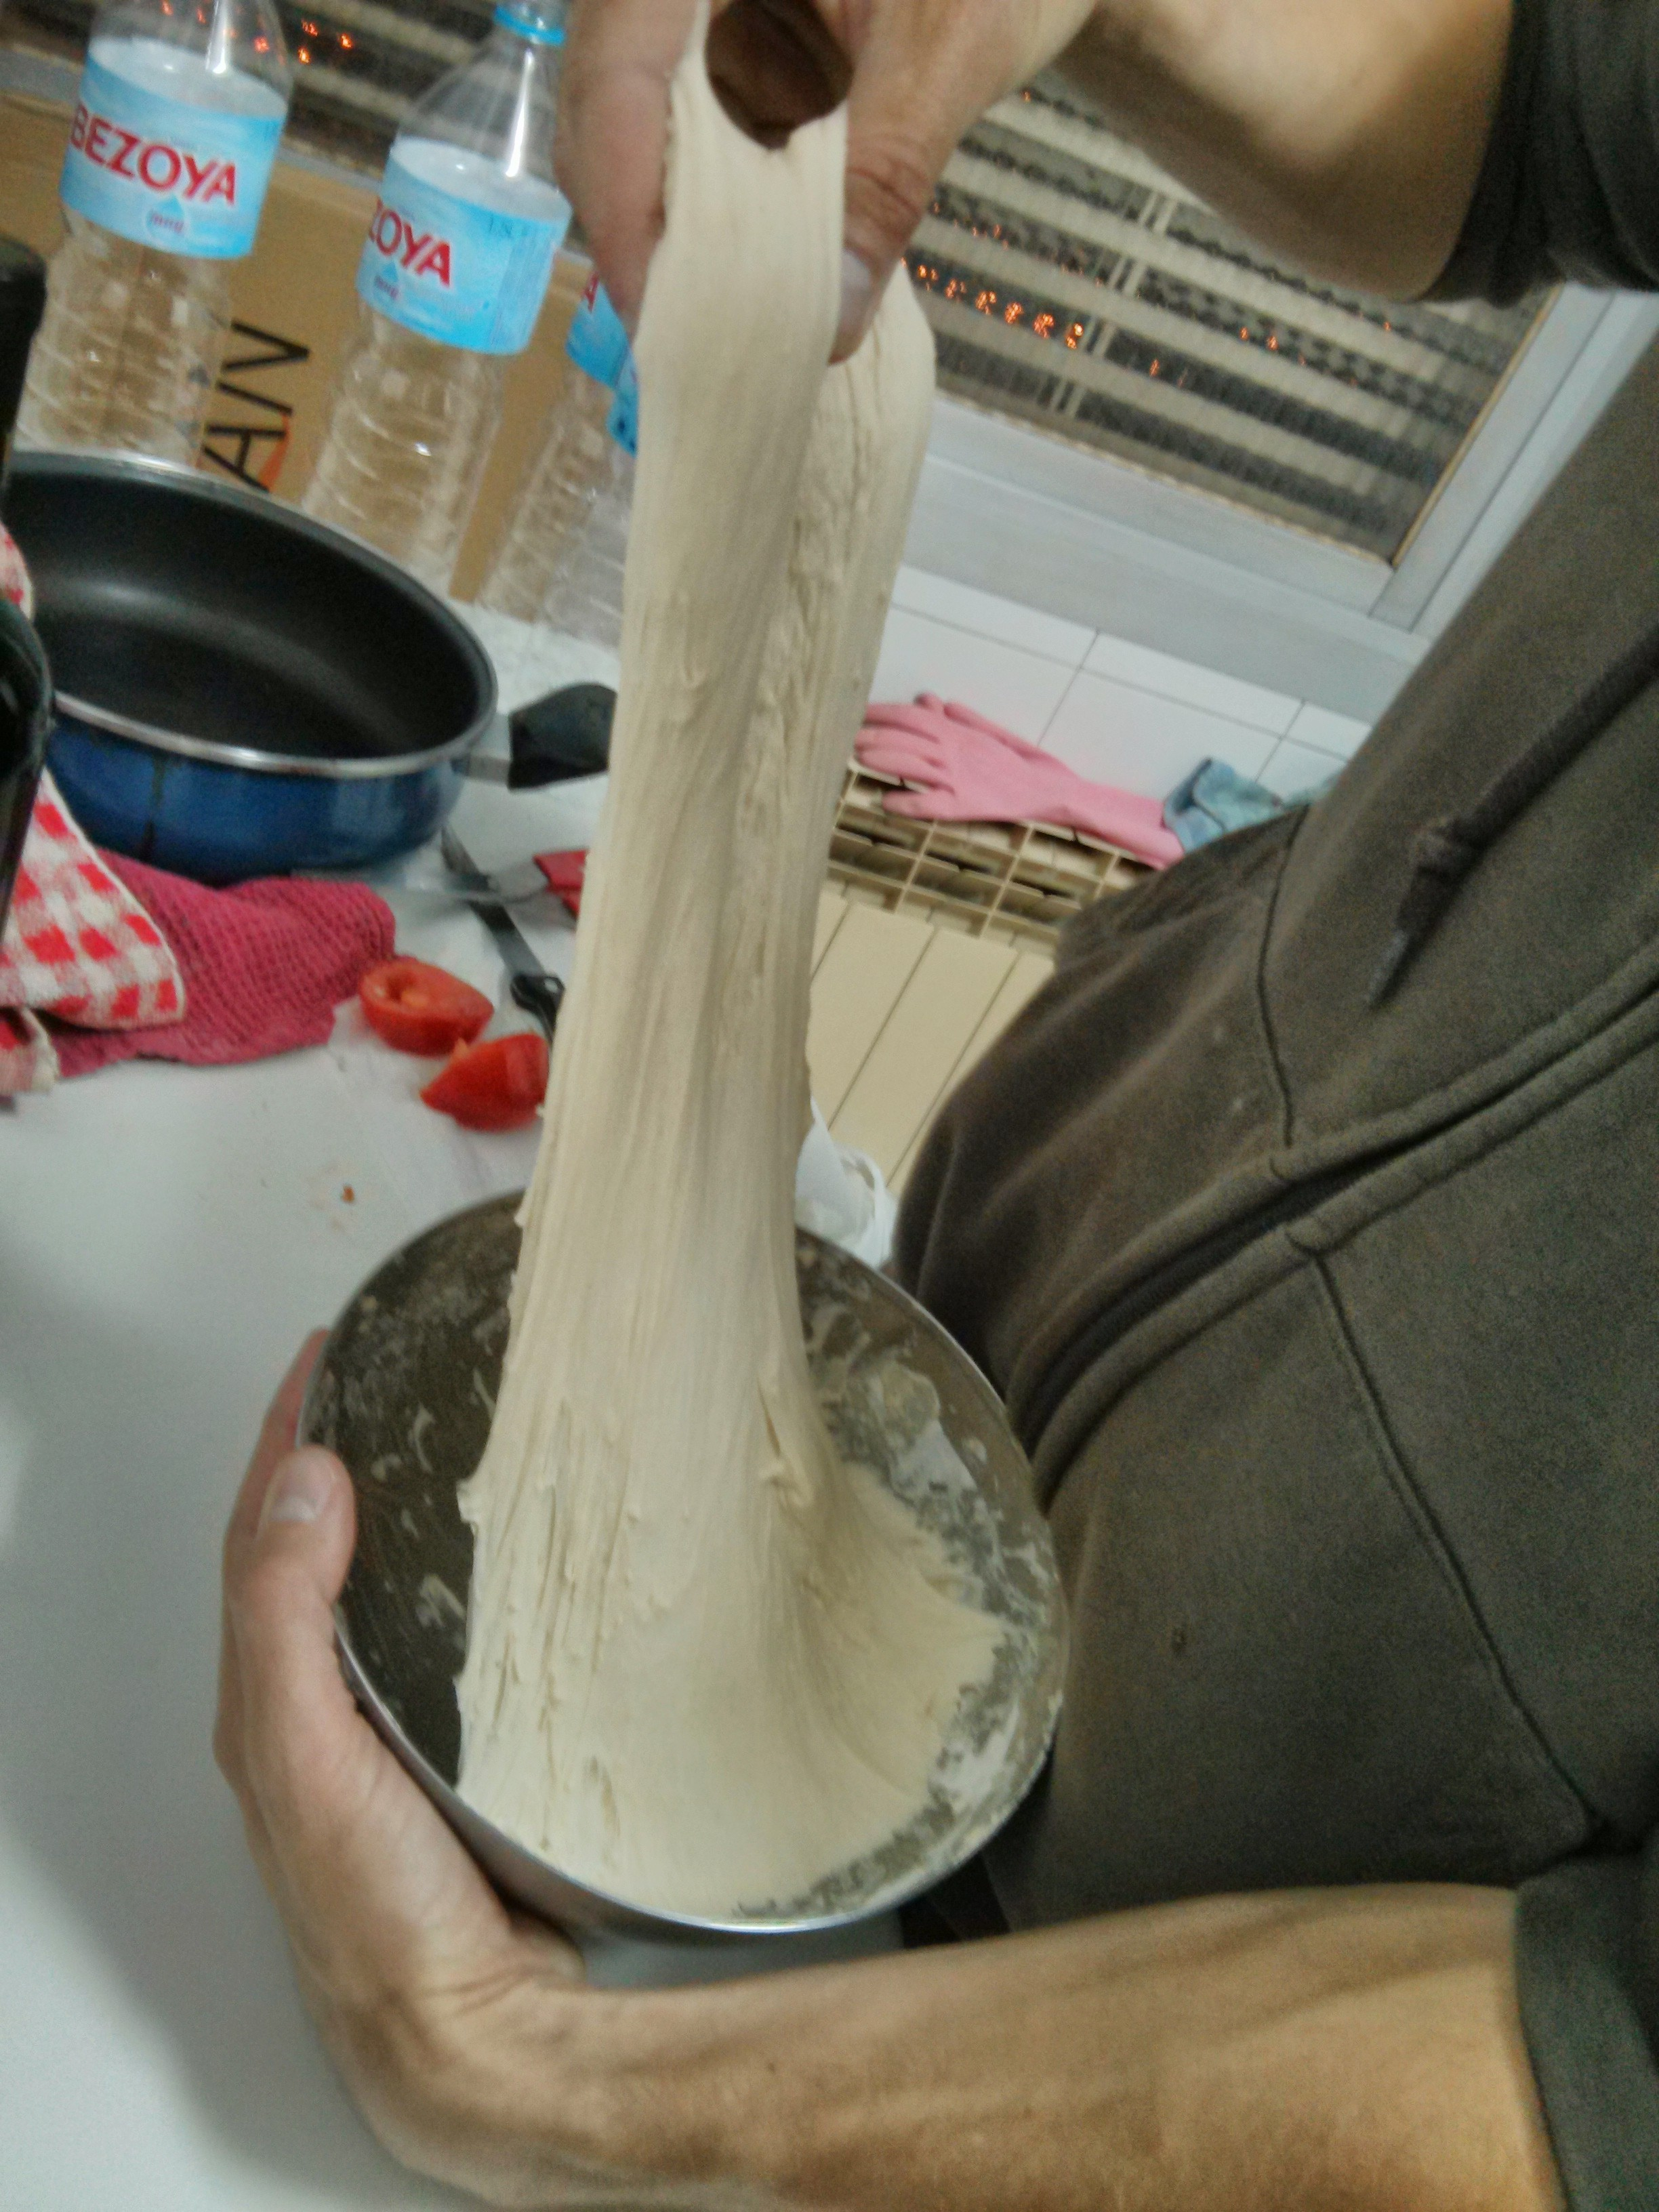
\includegraphics[width=0.5\linewidth]{estirar_massa}
            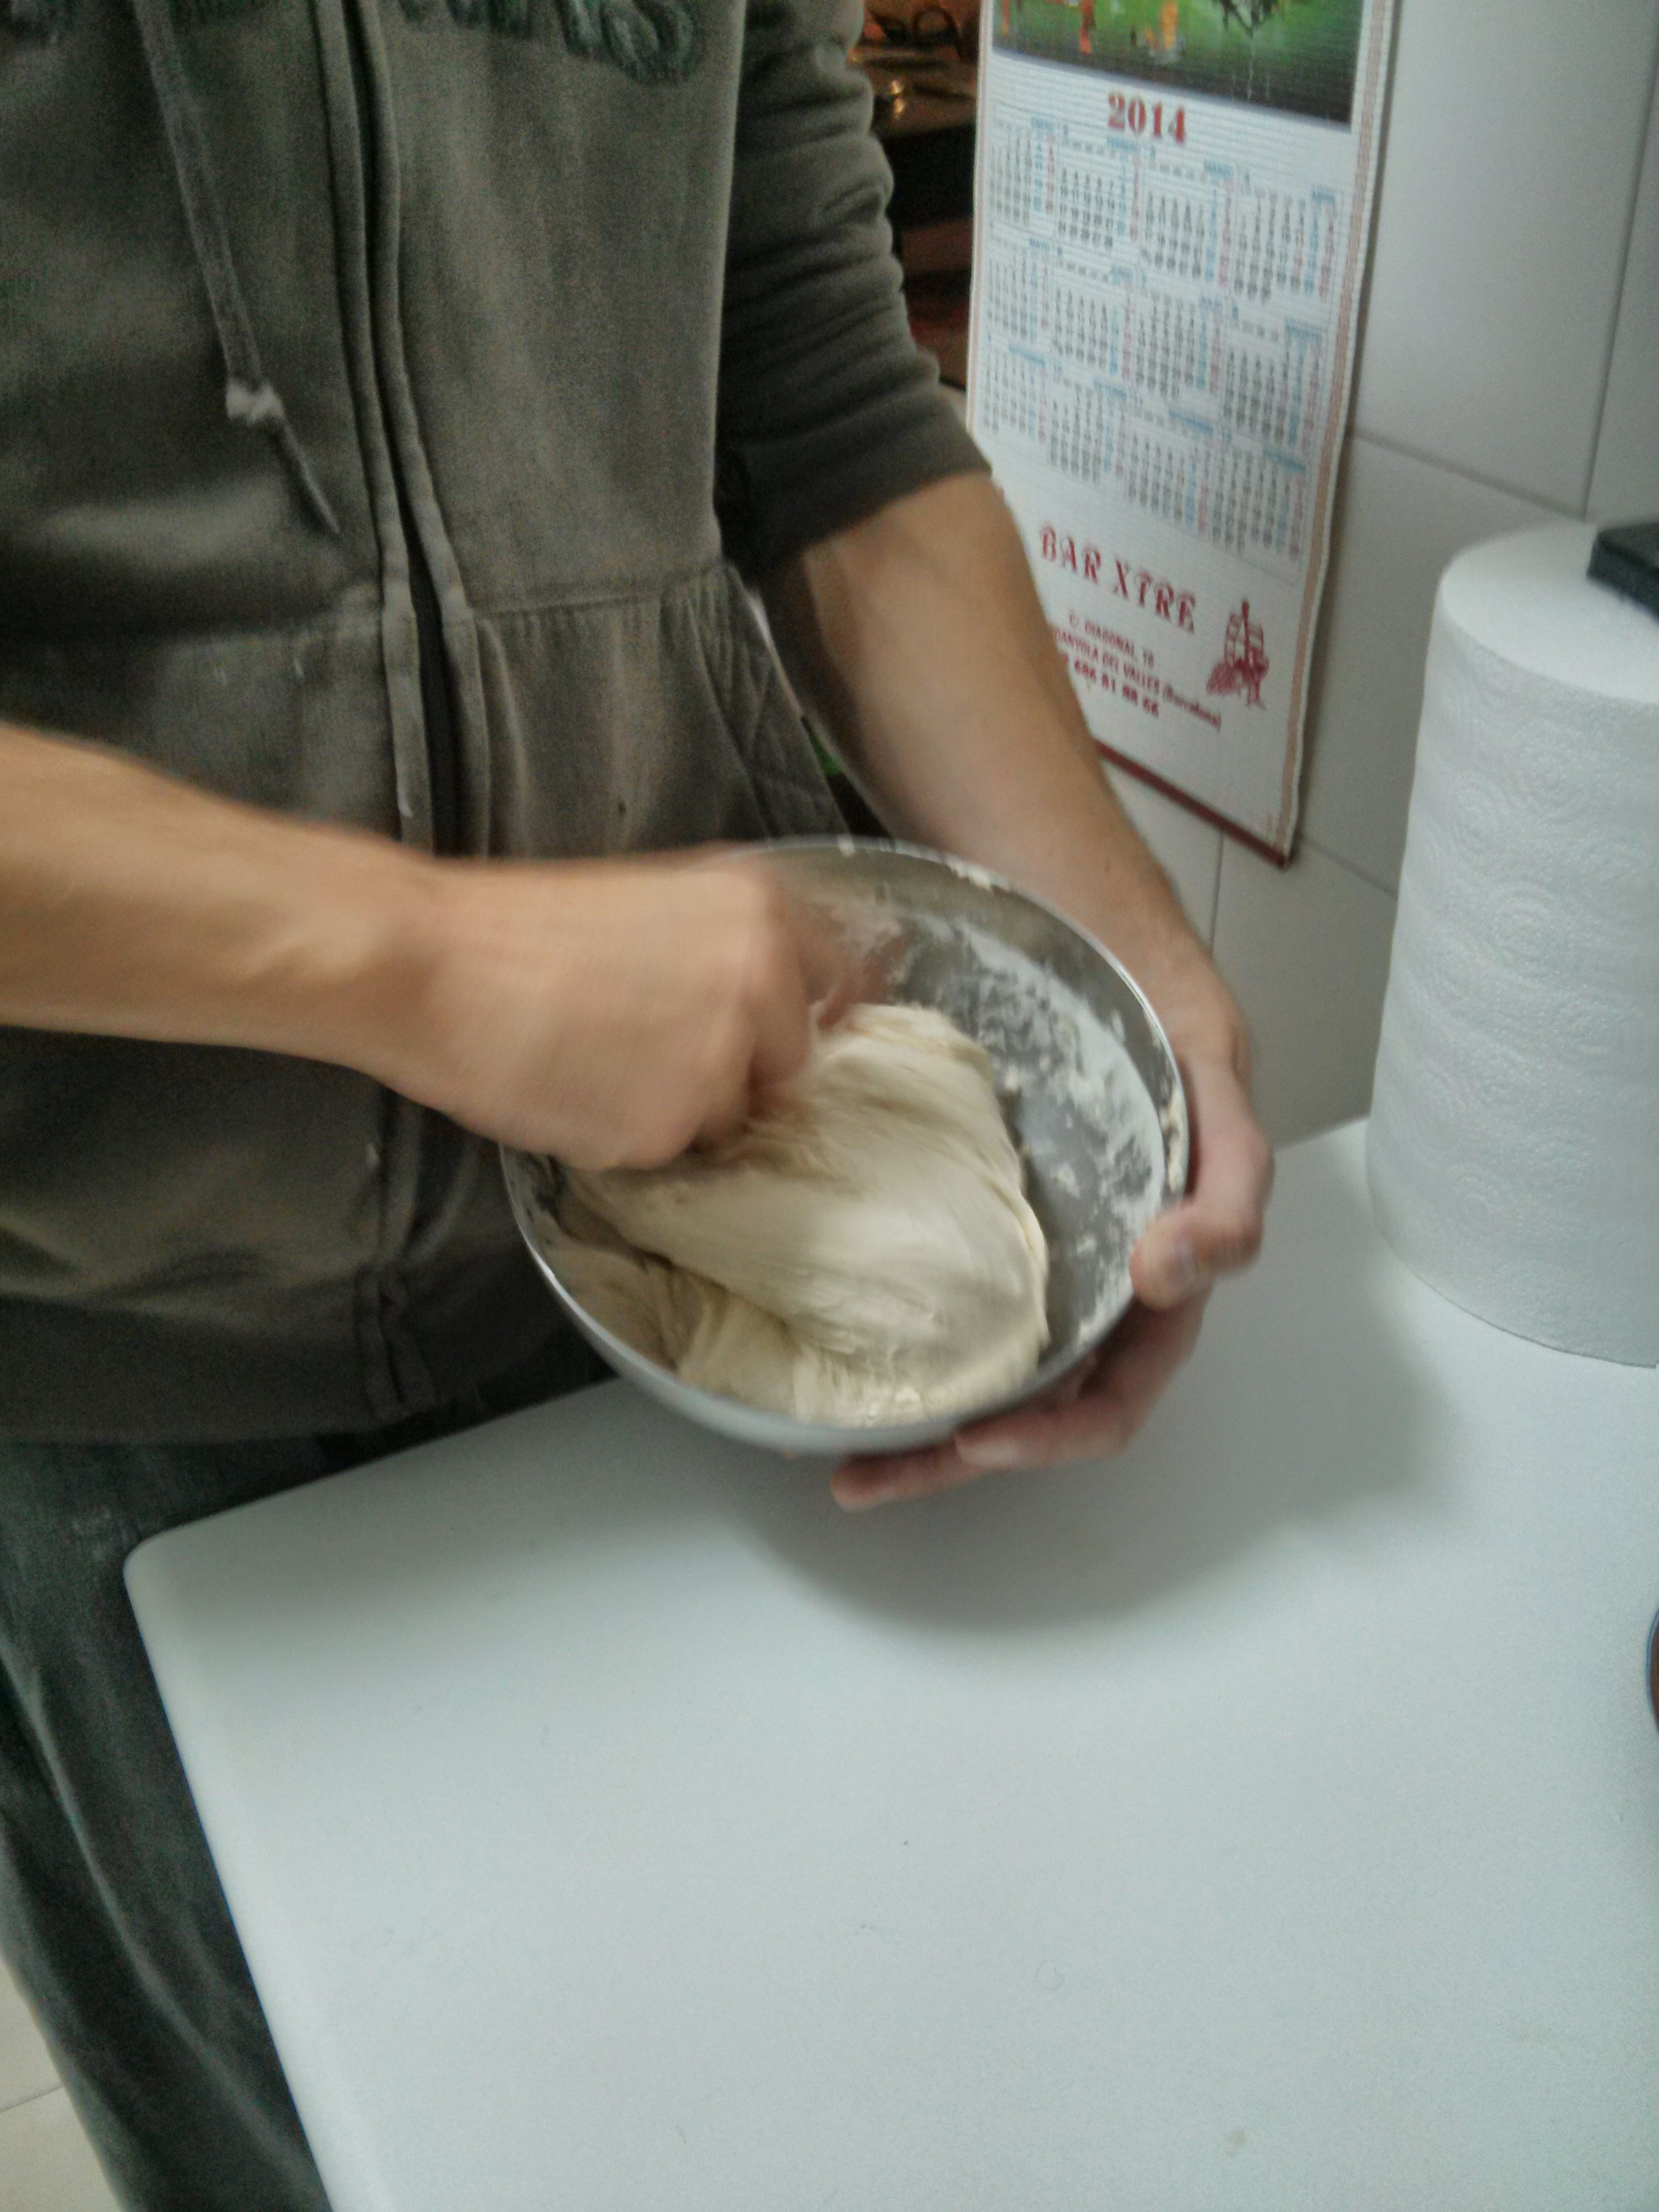
\includegraphics[width=0.5\linewidth]{plegar_massa}
		\end{figure}
        \end{center}\\
    
    	\hline

        
        \\Nevera
        
        &
        
        
        12$\approx$24 h.\\
        
        \hline
        
	\end{tabular}
	\end{table}

}
\end{frame}


%------------------------------------------------
% Table Crear
%------------------------------------------------

\fbckg{pa_fons.jpg}
\begin{frame}
\misc{

	\Huge Crear: \normalsize

	\begin{table}[ht]
	\centering
	\begin{tabular}{*{2}{m{0.48\textwidth}}}
    	\hline
        
        \begin{center}
        \begin{figure}[h]
			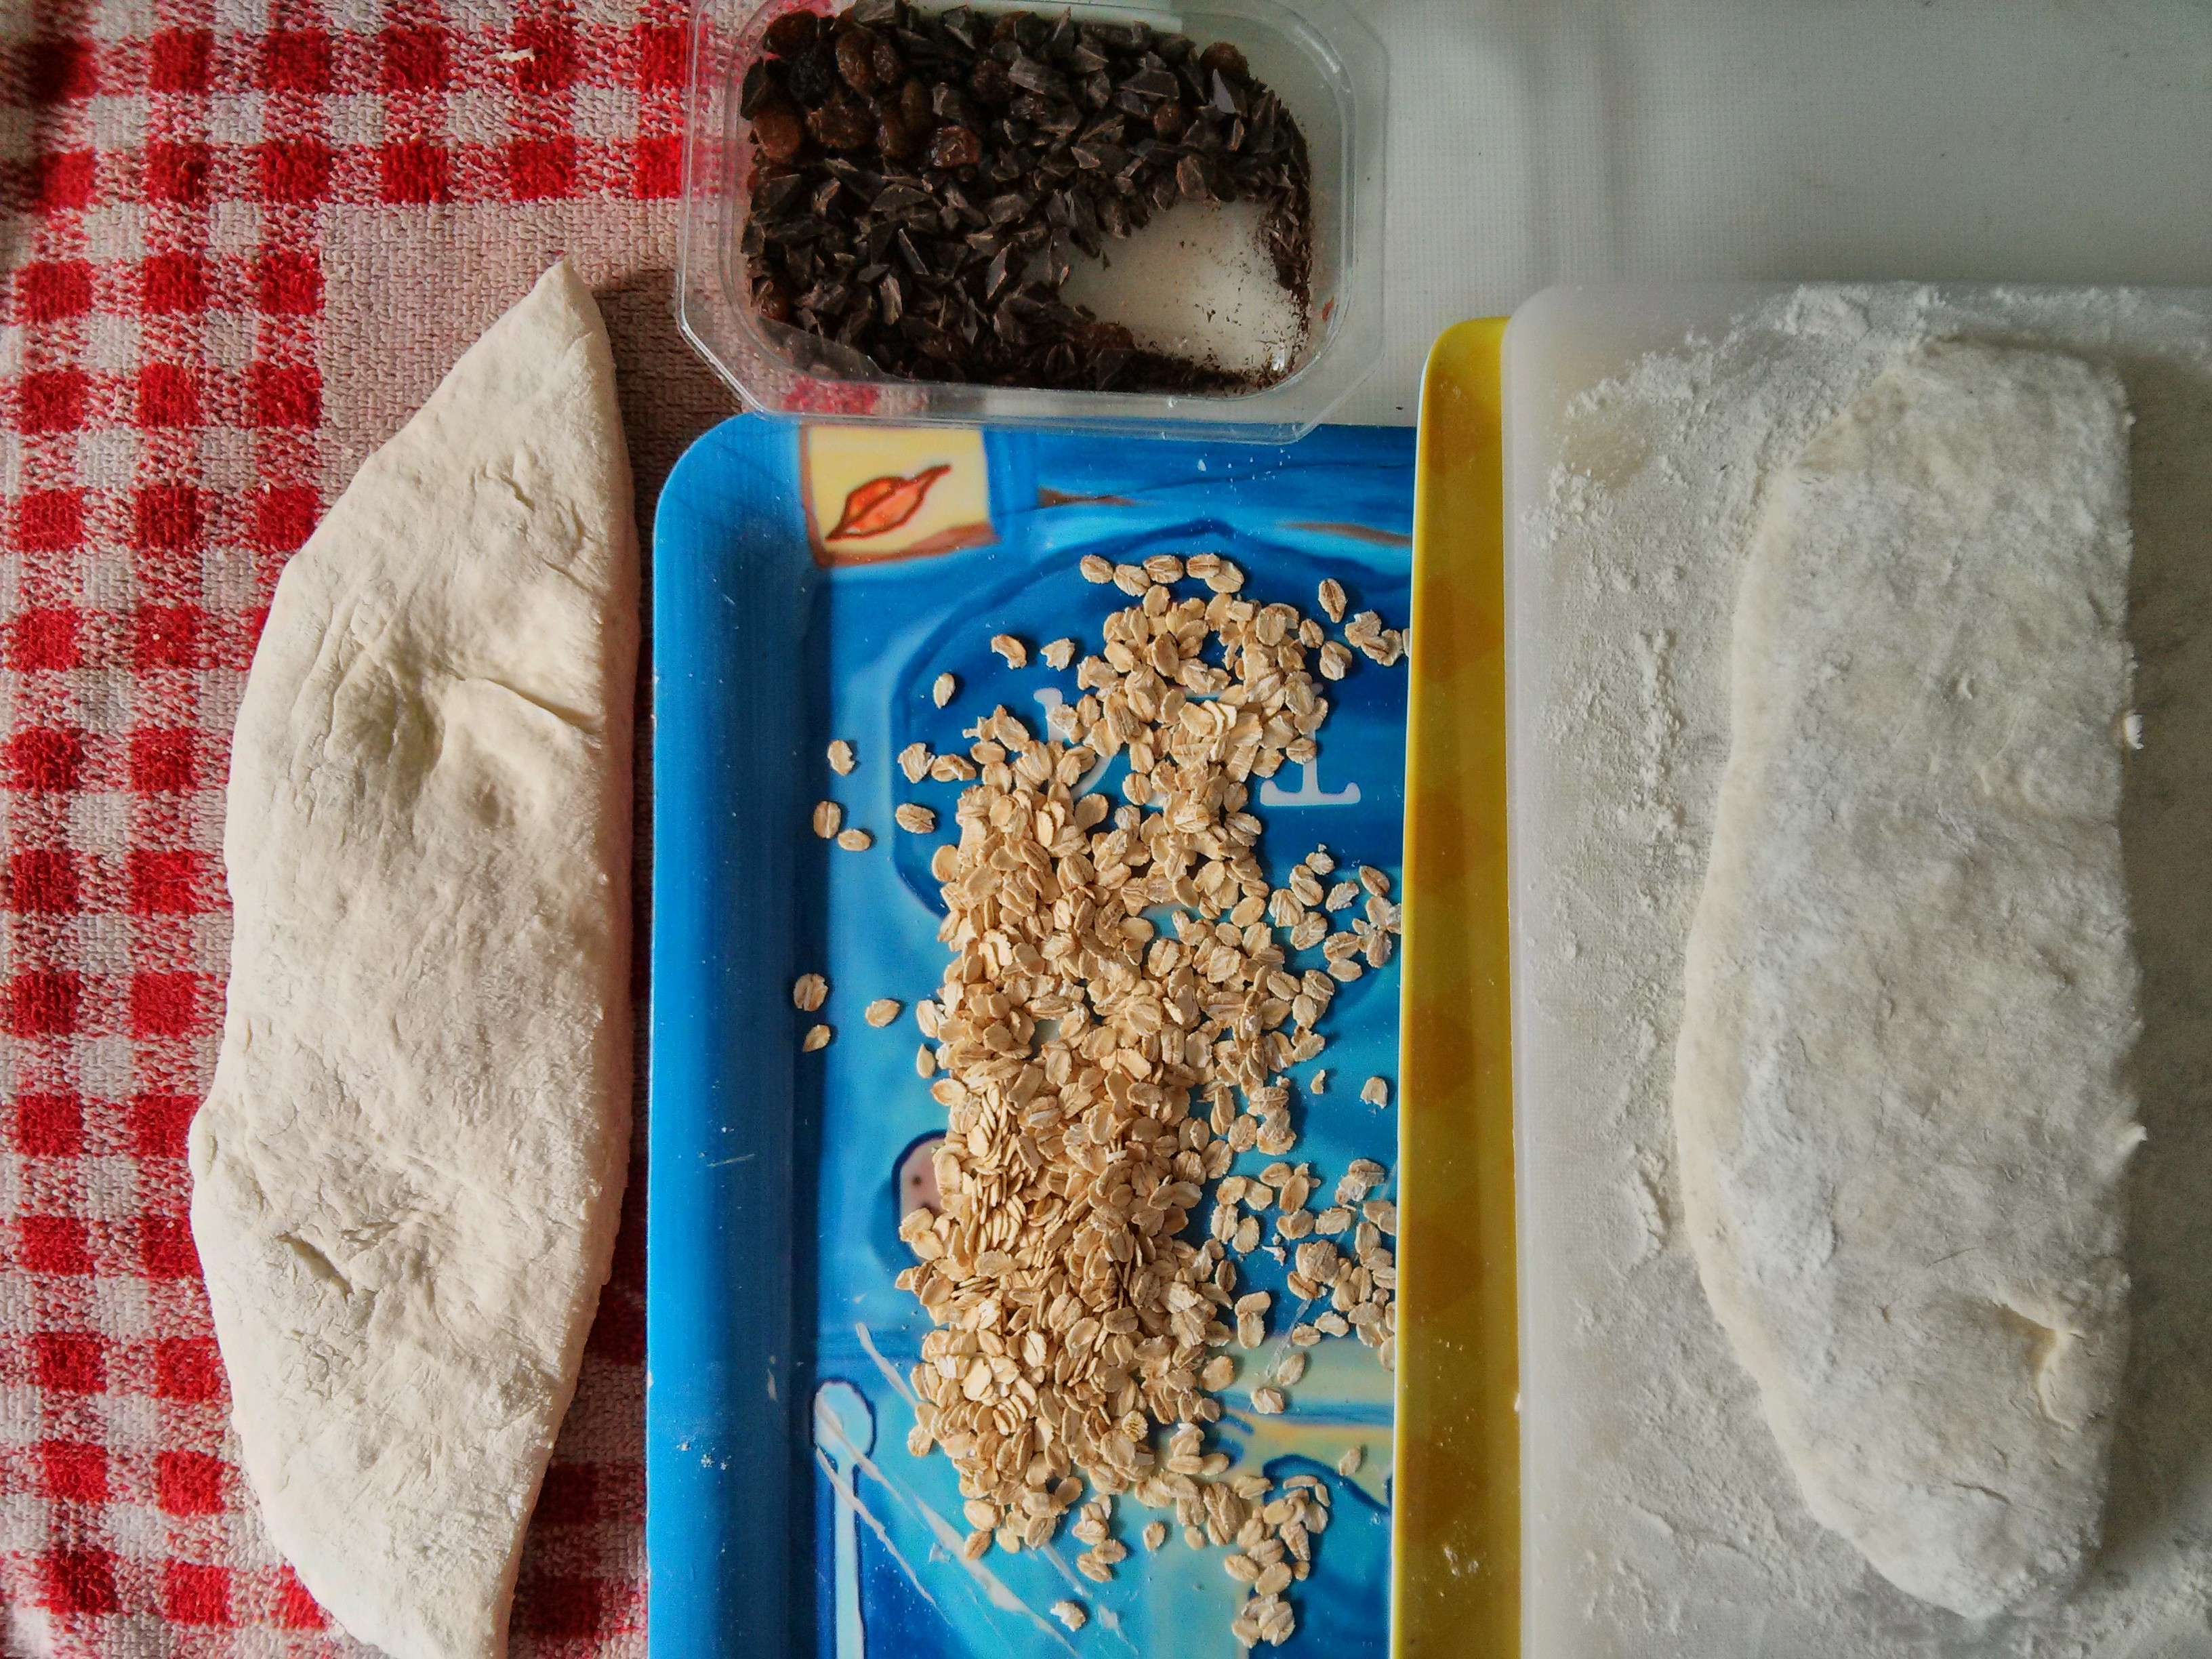
\includegraphics[width=1\linewidth]{crear}
		\end{figure}        
        \end{center}
        
        &
       
        \begin{itemize}
        	\item Palpar
        	\item Airear 1h. (opt)
        	\item Estendre
        	\item Tallar en 2
        	\item Humitejar
        	\item Sembrar
        	\item Trenar
        \end{itemize}
        \\
		
        \hline
        
	\end{tabular}
	\end{table}

} %misc
\end{frame}



%------------------------------------------------
% Table Fornejar
%------------------------------------------------

\fbckg{pa_fons.jpg}
\begin{frame}
\misc{

	\Huge Fornejar: \normalsize

	\begin{table}[ht]
	\centering
	\begin{tabular}{*{2}{m{0.48\textwidth}}}
		\hline
        
        \begin{itemize}
        	\item Preescalfar 250º C
        	\item Introduir + $1/2$ got H$_2$O
        	\item Apagar 10 min
        	\item Engegar 200º C
        	\item Fornejar 25$\approx$40 min.
        \end{itemize}
        
        &
        
        \begin{center}
        \begin{figure}[h]
			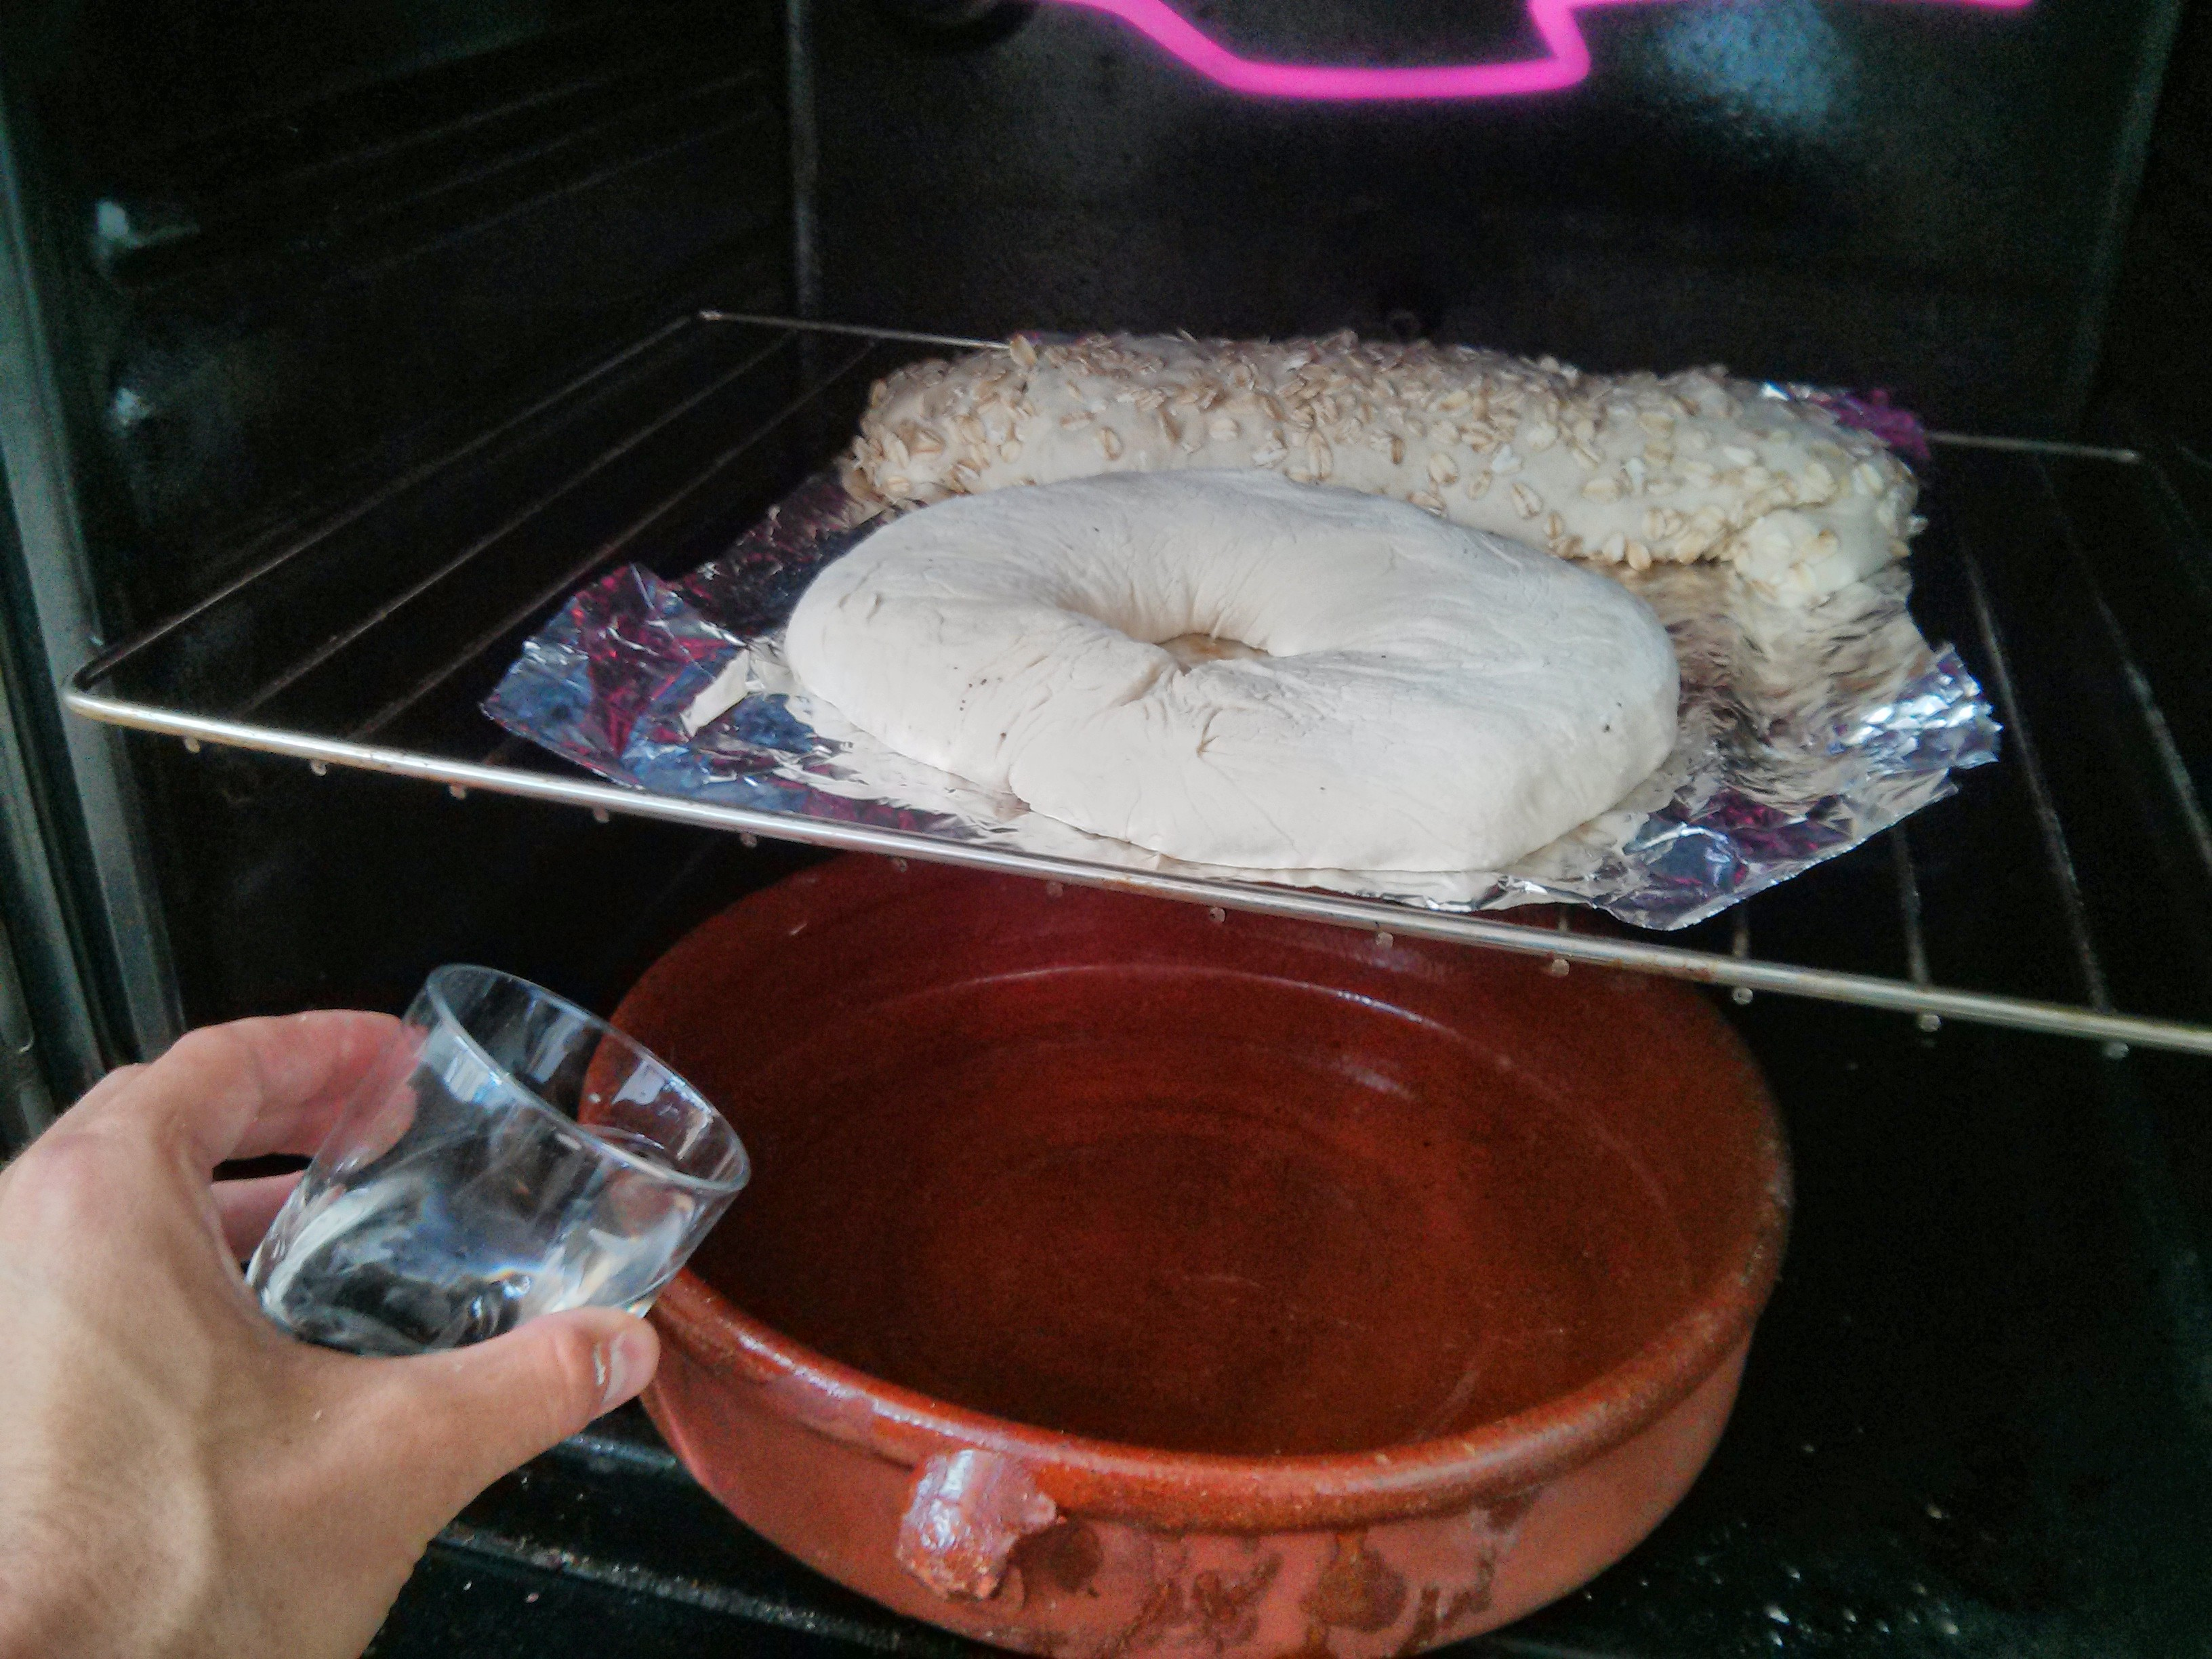
\includegraphics[width=1\linewidth]{fornejar}
		\end{figure}
        \end{center}
    	\\
        
        \hline
        
	\end{tabular}
	\end{table}

}
\end{frame}


%------------------------------------------------
% Resources
%------------------------------------------------

\fbckg{pa_fons}
\begin{frame}
\misc{
Resources:
\begin{figure}[h]
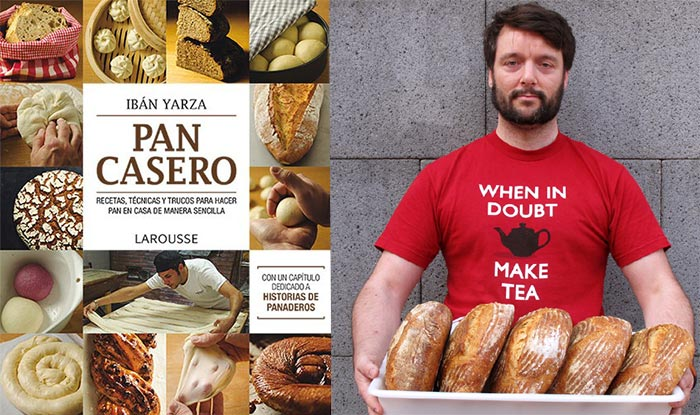
\includegraphics[width=0.4\linewidth]{Iban_pancasero}
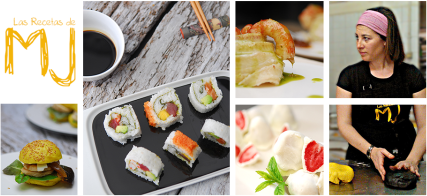
\includegraphics[width=0.52\linewidth]{LasRecetasDeMJ}
\end{figure}
Recepta: http://goo.gl/aFyLZS (Ib\'an Yarza \& Las Recetas de MJ)\\
elforodelpan.com\\
lamemoriadelpan.com\\
tequedasacenar.com\\

}
\end{frame}

%------------------------------------------------
% Thank you
%------------------------------------------------

\fbckg{mans_a_la_massa.jpg}
\begin{frame}
\thankyou % Inserts a thank you slide
\end{frame}



%------------------------------------------------
% Table
%------------------------------------------------

\fbckg{pa_fons.jpg}
\begin{frame}
\misc{
%Tables can be included with the \texttt{\textbackslash misc\{\}} command:
Trade-off
\begin{table}[h]
\begin{tabular}{l l l}
\toprule
\textbf{Pa amb:} & \textbf{Llevat} & \textbf{Massa madre}\\
\midrule
time & Rapid & Lento \\
top & Senzill & Elaborat \\
stdout & Bonn\'issim & Suprem \\
\bottomrule
\end{tabular}
\end{table}
}
\end{frame}

%------------------------------------------------
% Table
%------------------------------------------------

\fbckg{pa_fons.jpg}
\begin{frame}
\misc{


\$ \texttt{man Pa}\\

\begin{table}[h]
\begin{tabular}{l l l l}

	\toprule

	\textbf{(1)Amassar} & \textbf{(2)Nevera} & \textbf{(3)Crear} & \textbf{(4)Fornejar}\\

	\midrule

	Empaquetar & Nevera $12\approx24$ h. & Sentir & Preescalfar 250ºC\\
	Reposar 15\' &  & Airejar 1h. (opt) & Meter + $1/2$H$_2$O @ bandeja\\
	Empquetar(2) &  & Estendre & Apagar 10m\\
	Reposar 15\' &  & Tallar en 2 & Engegar 200º\\
	Empquetar(3) &  & Humitejar & Fornejar $25\approx40$m\\
	Reposar 15\' &  & Sembrar & \\
	Empquetar(4) &  & Trenar & \\


	\bottomrule
\end{tabular}
\end{table}
}
\end{frame}


%----------------------------------------------------------------------------------------

\end{document}
